% Dokumentklassen sættes til memoir.
% Manual: http://ctan.org/tex-archive/macros/latex/contrib/memoir/memman.pdf
\documentclass[a4paper,oneside,article]{memoir}

% Danske udtryk (fx figur og tabel) samt dansk orddeling og fonte med
% danske tegn. Hvis LaTeX brokker sig over æ, ø og å skal du udskifte
% "utf8" med "latin1" eller "applemac". 
\usepackage[utf8]{inputenc}
\usepackage[danish]{babel}
\usepackage{kpfonts}
\usepackage{float}

% Matematisk udtryk, fede symboler, theoremer og fancy ting (fx kædebrøker)
\usepackage{amsmath,amssymb}
\usepackage{bm}
\usepackage{amsthm}
\usepackage{mathtools}
\usepackage{gensymb}

\usepackage{hyperref}

% Kodelisting. Husk at læse manualen hvis du vil lave fancy ting.
% Manual: http://mirror.ctan.org/macros/latex/contrib/listings/listings.pdf
\usepackage{listings}

% Fancy ting med enheder og datatabeller. Læs manualen til pakken
% Manual: http://www.ctan.org/tex-archive/macros/latex/contrib/siunitx/siunitx.pdf
\usepackage{siunitx}

% Indsættelse af grafik.
\usepackage{graphicx}

\usepackage{braket}
\usepackage{caption}



% Reaktionsskemaer. Læs manualen for at se eksempler.
% Manual: http://www.ctan.org/tex-archive/macros/latex/contrib/mhchem/mhchem.pdf
\usepackage[margin=0.9in]{geometry}

\usepackage[version=3]{mhchem}

\usepackage{units}

\newcommand{\dif}[1]{\frac{d}{d {#1}}}

\newcommand{\mylim}[2]{\lim\limits_{#1 \rightarrow #2}}

\newcommand{\myset}[2]{\left\{ #1 \mid #2 \right\} }

\newcommand{\funkt}[3]{#1 : #2 \rightarrow #3}

\newcommand{\funktt}[3]{#1 : #2 \rightarrow \mathbb{#3}}

\DeclareMathOperator{\Span}{Span}
\DeclareMathOperator{\sd}{sd}
\DeclareMathOperator{\Var}{Var}
\DeclareMathOperator{\Det}{Det}
\DeclareMathOperator{\Mat}{Mat}
\DeclareMathOperator{\Geo}{Geo}

\newenvironment{amatrix}[1]{%
  \left(\begin{array}{@{}*{#1}{c}|c@{}}
}{%
  \end{array}\right)
}

\parindent=0pt

\usepackage[framed,numbered,autolinebreaks,useliterate]{mcode}

\begin{document}

\title{Adgangsspørgsmål til Fysik Camp 2018}

\author{Fagligt Team}

\maketitle

%\textbf{Matematik}\\
%Gradienten for en funktion $f(x,y,z)$ er defineret som,
%\begin{align*}
%\nabla f(x,y,z) = \left( \frac{\partial f(x,y,z)}{\partial x}, \frac{\partial f(x,y,z)}{\partial y}, \frac{\partial f(x,y,z)}{\partial z} \right)
%\end{align*}
%hvor $\frac{\partial f(x,y,z)}{\partial x}, \frac{\partial f(x,y,z)}{\partial y}, \frac{\partial f(x,y,z)}{\partial z}$ er de partielt afledte mht. til henholdsvis $x,y$ og $z$. Når man udregner en den partielt afledte for en funktion af flere variable, differentier man mht. en variabel imens man holder de resterende konstante.\\
%
%a) Udregn gradienten af funktionen $g(x,y,z)=2xy+z^2$.\\
%
%
%b) I dine egne ord, hvad er det så gradienten fortæller os om funktionen \indent$g(x,y,z)$?\\

\textbf{Spørgsmål 1}\\
Du har en klods på et skråplan. Klodsen er placeret i højden $h$ fra jordoverfladen.\\

a) Hvilke kræfter kan virke på klodsen?\\

Antag nu, at den mekaniske energi er bevaret, således at den er den samme under hele klodsens tur ned af skråplanet, og er givet ved $E = \tfrac{1}{2} mv^2 + mgh$. Til at starte med er klodsen i hvile (dvs. $v=0$) på skråplanet i højden $h$ fra jordoverfladen.\\

b) Hvad er farten $v$ af klodsen udtrykt ved de andre parametre fra energien $E$, når den når bunden af skråplanet?\\

c) Antag, at $g = 10$ m/s, og $h = 5$ m. Hvad er $v$ så ved bunden af skråplanet?\\

\begin{figure}[h!]
	\centering
	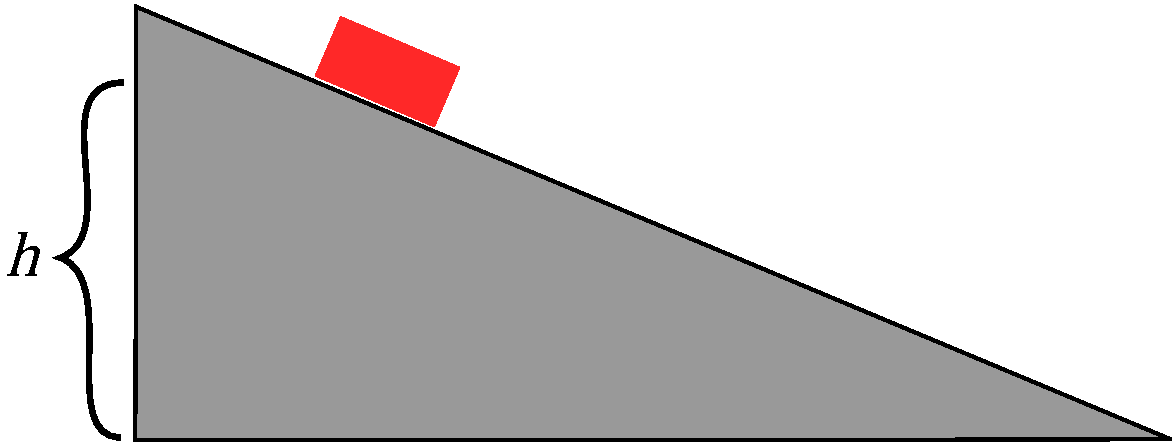
\includegraphics[scale=0.6]{figur_ana.pdf}
\end{figure}

\textbf{Spørgsmål 2}\\
Hvad er partikel-bølge dualiteten? Forklar det kort med dine egne ord.\\


\textbf{Spørgsmål 3}\\
Hvilke egenskaber ville du kigge efter, hvis du skulle vælge den næste planet, menneskeheden skulle bosætte sig på? Beskriv kort hvorfor.\\

\textbf{Spørgsmål 4}\\
En satellit kredser i en cirkulær bane omkring jorden. Den påvirkes udelukkende af en tiltrækkende tyngdekraft fra jorden, som er givet ved $F_g = GMm/r^2$, hvor $M$ er jordens masse, $m$ er satellittens masse, $G$ er gravitationskonstanten og $r$ er afstanden fra jordens centrum til satellitten.\\

a) Hvis satellitten er i en afstand $r = 8000$ km fra jordens centrum, og jordens masse er $M = 6 \times 10^{24}$ kg, hvor stor en fart $v$ må den så have for at kunne bibeholde den cirkulære bevægelse omkring jorden?\\

Hint: For at et objekt kan opretholde en cirkulære bevægelse, skal der være en kraft (her er det tyngdekraften), som virker på objektet ind mod centrum af cirkelbevægelsen. Sådan en kraft kaldes en centripetalkraft, og størrelsen af denne kan altid skrives som $F_c = mv^2/r$, hvor $m$ er objektets masse, $v$ dets fart og $r$ er afstanden fra objektet til centrum af cirkelbevægelsen.\\

\textbf{Spørgsmål 5}\\
Hvad synes du, er det fedeste ved fysik? Skriv maximum 10 linjer.

%\textbf{Geometrisk Optik}\\
%I denne opgave skal du kigge på en lysstråle, der bevæger sig, som det er vist på figuren. For at løse opgaven skal du bruge to resultater, der forklarer, hvordan en lysstråle opfører sig ved refleksion og refraktion. Det første resultat siger, at ved refleksion er indgangsvinklen ift. refleksionsoverfladens normal den samme som udgangsvinkelen ift. normalen. Det andet resultat kaldes for Snells lov og siger, at ved refraktion er forholdet mellem indgangsvinklen og udgangsvinklen (stadig ift. normalen) givet ved formlen $n_1 \sin \theta_1 = n_2 \sin \theta_2$, hvor $n_1$ og $n_2$ er brydningsindekser. Endeligt skal der også bruges lidt trigonometri, og de nødvendige formler kan findes på følgende link: \url{http://www.webmatematik.dk/lektioner/matematik-c/trigonometri/cosinus-sinus-og-tangens-i-retvinklede-trekanter}.\\
%
%I opgaven sættes $n_a = 1$, $a=$\SI[mode=text]{10}{\centi\meter} og $b=$\SI[mode=text]{15}{\centi\meter}.\\
%
%a) Hvad skal $\theta_a$ være, så lyset rammer siden med længden $b$ præcist på midten?\\
%
%b) Find et udtryk for $\theta_d$ som funktion af $\theta_a$ (Hint: Start med at finde et udtryk for $\theta_b$ som funktion af $\theta_a$. Find så et udtryk for $\theta_c$ som funktion af $\theta_b$. Endeligt, find et udtryk for $\theta_d$ som funktion af $\theta_c$.). \\
%
%c) Hvad skal $n_b$ være, hvis $\theta_d = \theta_a / 2$, hvor $\theta_a$ er vinklen fundet i spørgsmål a)?
%
%\begin{figure}[h!]
%	\centering
%	\includegraphics[scale=0.7]{figur.pdf}
%\end{figure}

\end{document}